\begin{figure}
    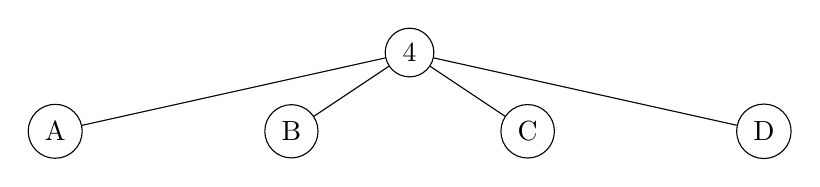
\begin{tikzpicture}
        \tikzstyle{every node}=[circle, draw];
        \draw (0,0) node (root) [anchor=south] {4} child {node {A}} child {node {B}} child {node {C}} child {node {D}};
            
    \end{tikzpicture}
    \caption*{Flat access tree}
\end{figure}


\begin{figure}
    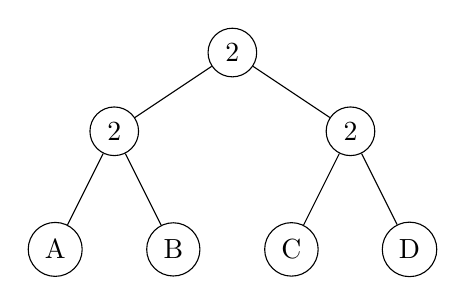
\begin{tikzpicture}
        \tikzstyle{every node}=[circle, draw];
        \tikzstyle{level 1}=[sibling distance=3cm, level distance=1cm];
        \tikzstyle{level 2}=[sibling distance=1.5cm, level distance=1.5cm];
        \draw (0,0) node (root) [anchor=south] {2} child {node {2} child {node {A}} child  {node {B}}} child {node {2} child {node {C}} child  {node {D}}};
    \end{tikzpicture}
    \caption*{Perfect binary access tree}
\end{figure}